\documentclass[10pt,a4paper]{article}

\usepackage[T1]{fontenc}
\usepackage{lmodern}
\usepackage[a4paper,top=16mm,bottom=16mm,left=20mm,right=20mm]{geometry}
\usepackage{amsmath,amssymb}
\usepackage{booktabs}
\usepackage[expansion=false]{microtype}
\usepackage{xcolor}
\usepackage{tikz}
\usetikzlibrary{arrows.meta,positioning,calc,decorations.pathreplacing}
\usepackage[hidelinks]{hyperref}
\hypersetup{pdftitle={A Dot Product Is All You Need},pdfauthor={Emad Mostaque}}

\definecolor{bandfill}{HTML}{EEF3F8}
\definecolor{bandedge}{HTML}{B9C9DC}
\definecolor{boxfill}{HTML}{FFFFFF}
\definecolor{boxedge}{HTML}{5C7A99}
\definecolor{accent}{HTML}{2B5B84}
\definecolor{rulecol}{HTML}{3B6E9C}

\setlength{\parindent}{1.2em}
\setlength{\parskip}{0pt}

\makeatletter
\renewcommand\section{\@startsection{section}{1}{\z@}%
  {-1.5ex \@plus -0.25ex \@minus -0.2ex}%
  {0.65ex \@plus 0.15ex}%
  {\normalfont\large\bfseries}}
\g@addto@macro\normalsize{%
  \setlength{\abovedisplayskip}{4.1pt \@plus 1.5pt \@minus 1.5pt}%
  \setlength{\belowdisplayskip}{4.1pt \@plus 1.5pt \@minus 1.5pt}%
  \setlength{\abovedisplayshortskip}{2.6pt \@plus 1pt \@minus 1pt}%
  \setlength{\belowdisplayshortskip}{2.6pt \@plus 1pt \@minus 1pt}%
}
\makeatother

\newcommand{\dd}{\mathrm{d}}
\newcommand{\R}{\mathbb{R}}
\newcommand{\C}{\mathbb{C}}
\newcommand{\E}{\mathbb{E}}
\newcommand{\hh}{\mathfrak{h}}
\newcommand{\HH}{\mathcal{H}}
\newcommand{\tr}{\operatorname{tr}}
\newcommand{\Dom}{\operatorname{Dom}}
\newcommand{\sinc}{\operatorname{sinc}}
\newcommand{\RePart}{\operatorname{Re}}
\newcommand{\ImPart}{\operatorname{Im}}

\begin{document}

\begin{center}
  {\LARGE A Dot Product Is All You Need\par}
  \vspace{0.7em}
  {\large Emad Mostaque\par}
{\small 26 November 2026\par}
\end{center}
\vspace{0.3em}

\begin{center}
\begin{minipage}{0.89\textwidth}
\small
\begin{center}\textbf{Abstract}\end{center}
\vspace{-0.4em}
\noindent This paper applies the axiomatic method to a mathematical question: what quantum structure does a positive dot product determine under the stated rules? The answer is the structure generated by a free scalar field. Only two scales remain free. The axiom is that displacements are measured by a single positive dot product $g$ in dimension $D \ge 2$. Squared lengths of orthogonal parts add, and this equation is read twice. With the product rule it makes scalar readings jointly Gaussian; with the sum rule it gives the Born rule. For readings smoother than white noise, maximizing entropy at the specified site and edge moments fixes a reflection-positive law with degree-one precision and covariance $\hbar(-\Delta_g + m^2)^{-1}$ and scales $m, \hbar > 0$. A state is what a plane knows of its preparation: the state space is the $L^2$ space of the field on the plane, a Fock space where the shift continues uniquely to unitary evolution $e^{-itH/\hbar}$, $H \ge 0$, and rotations continue to Lorentz boosts. The product rule gives the tensor product and the update. The von Neumann and Wightman axioms follow.
\end{minipage}
\end{center}
\vspace{0.2em}

\section{The axiom}

\noindent\textbf{Axiom.} \textit{Displacements are measured by a single positive dot product $g$.}

\medskip
Fix a real affine space of dimension $D \ge 2$. The dot product on its translation space determines lengths, orthogonality, reflections and a Laplacian $\Delta_g$. A \textit{reading} is a number $\Phi(f) = \int f\varphi$, a real scalar field $\varphi$ sampled by a real Schwartz test function $f$. The axiom fixes the geometry, not the readings: a statement about them carries a probability, and the joint distribution of every finite list of readings is the \textit{law}. Which law does the axiom determine?

What the axiom leaves open is governed by probability: its sum and product rules, symmetry, and maximum entropy. By the axiomatic method nothing else is assumed; Figure~1 shows where each is used. For readings these say:

\begin{list}{}{%
  \setlength{\leftmargin}{1.35em}%
  \setlength{\itemsep}{0.16em}%
  \setlength{\parsep}{0pt}%
  \setlength{\topsep}{0.32em}%
}
\item \textbf{Sum rule.} Laws are nonnegative, normalized and countably additive on exclusive (orthogonal) events; a sublist has the marginal law.
\item \textbf{Product rule.} Independently prepared parts multiply; selecting an event makes it certain and keeps the ratios of its subevents.
\item \textbf{Equal values.} Equivalent descriptions receive equal values: those related by isometries of $g$, of the covariance form and of the state space.
\item \textbf{Maximum entropy.} Given the lattice site and edge-difference mean squares (\S2.3), the law maximizes entropy, assuming nothing else.
\end{list}

\vspace{0.2em}
\noindent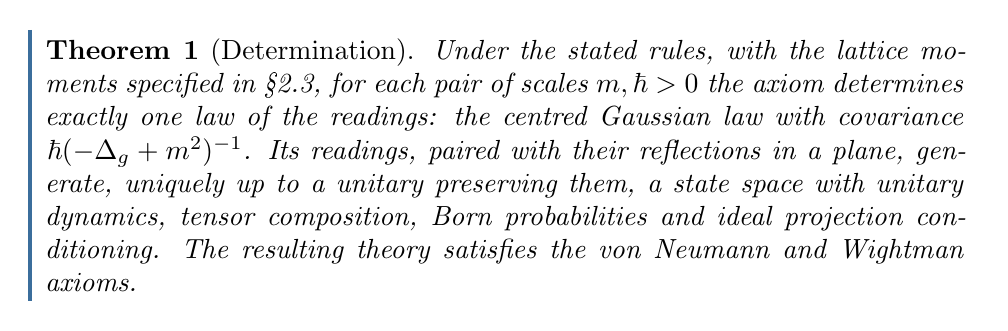
\begin{tikzpicture}[baseline=(box.base)]
\node[inner xsep=6pt, inner ysep=3pt, text width=\dimexpr\textwidth-14pt\relax, align=justify] (box) {%
  \textbf{Theorem 1} (Determination). \textit{Under the stated rules, with the lattice moments specified in~\S2.3, for each pair of scales $m, \hbar > 0$ the axiom determines exactly one law of the readings: the centred Gaussian law with covariance $\hbar(-\Delta_g + m^2)^{-1}$. Its readings, paired with their reflections in a plane, generate, uniquely up to a unitary preserving them, a state space with unitary dynamics, tensor composition, Born probabilities and ideal projection conditioning. The resulting theory satisfies the von Neumann and Wightman axioms.}%
};
\draw[rulecol, line width=1.6pt] (box.north west) -- (box.south west);
\end{tikzpicture}

\begin{figure}[!h]
\vspace{-0.2em}
\centering
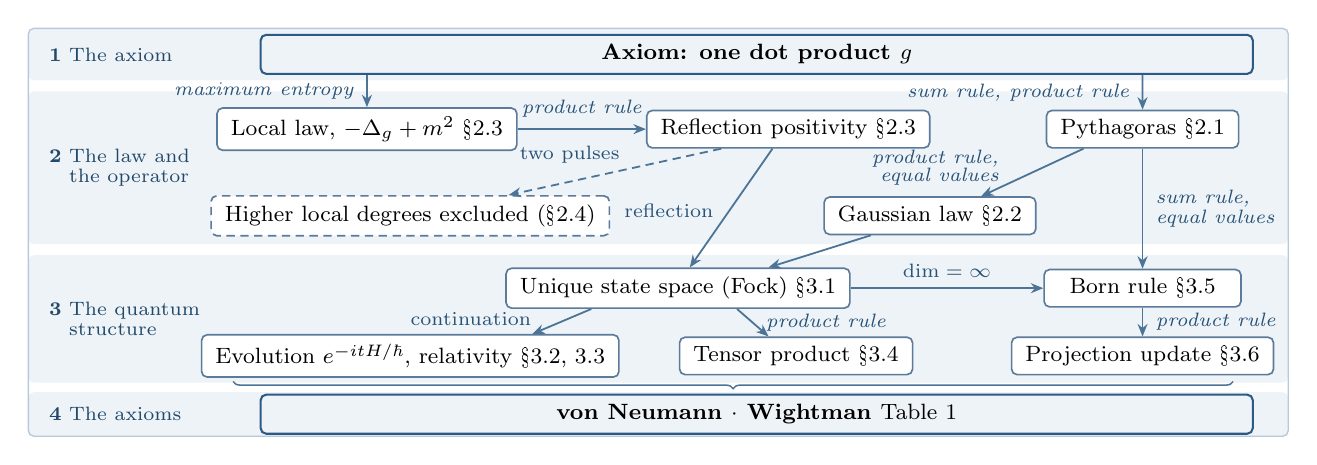
\begin{tikzpicture}[
  font=\footnotesize,
  nodebox/.style={draw=boxedge, fill=boxfill, rounded corners=2pt, inner xsep=5pt, inner ysep=3.2pt, line width=0.6pt, align=center},
  topbox/.style={draw=accent, fill=bandfill, rounded corners=2pt, inner xsep=7pt, inner ysep=3.5pt, line width=0.75pt, font=\footnotesize\bfseries, align=center},
  arr/.style={-{Stealth[length=4.5pt,width=3.6pt]}, draw=accent!85, line width=0.65pt},
  lbl/.style={font=\scriptsize\itshape, text=accent!90!black, inner sep=1.5pt},
  rlbl/.style={font=\scriptsize, text=accent!90!black, inner sep=1.5pt},
  bandlbl/.style={font=\scriptsize, text=accent!80!black, align=left, anchor=west}
]
  % Shaded horizontal bands
  \fill[bandfill, rounded corners=2pt] (0, 4.46) rectangle (16.0, 5.12);
  \fill[bandfill, rounded corners=2pt] (0, 2.38) rectangle (16.0, 4.32);
  \fill[bandfill, rounded corners=2pt] (0, 0.62) rectangle (16.0, 2.24);
  \fill[bandfill, rounded corners=2pt] (0, -0.06) rectangle (16.0, 0.50);

  \draw[bandedge, line width=0.5pt, rounded corners=2pt] (0, -0.06) rectangle (16.0, 5.12);

  % Band labels
  \node[bandlbl] at (0.14, 4.79) {\textbf{1} The axiom};
  \node[bandlbl] at (0.14, 3.35) {\textbf{2} The law and\\[-1pt]\phantom{\textbf{2} }the operator};
  \node[bandlbl] at (0.14, 1.43) {\textbf{3} The quantum\\[-1pt]\phantom{\textbf{3} }structure};
  \node[bandlbl] at (0.14, 0.22) {\textbf{4} The axioms};

  % Band 1 sole axiom node
  \node[topbox, minimum width=12.6cm] (axiom) at (9.25, 4.79) {Axiom: one dot product $g$};

  % Band 2 nodes
  \node[nodebox] (loc)  at (4.30, 3.84) {Local law, $-\Delta_g + m^2$ \S2.3};
  \node[nodebox] (rp)   at (9.65, 3.84) {Reflection positivity \S2.3};
  \node[nodebox] (pyth) at (14.15, 3.84) {Pythagoras \S2.1};

  \node[nodebox, densely dashed] (op) at (4.85, 2.74) {Higher local degrees excluded (\S2.4)};
  \node[nodebox] (gauss) at (11.45, 2.74) {Gaussian law \S2.2};

  % Band 3 nodes
  \node[nodebox, minimum width=4.3cm] (fock) at (8.25, 1.82) {Unique state space (Fock) \S3.1};
  \node[nodebox, minimum width=2.5cm] (born) at (14.15, 1.82) {Born rule \S3.5};

  \node[nodebox] (evol) at (4.85, 0.96) {Evolution $e^{-itH/\hbar}$, relativity \S3.2, 3.3};
  \node[nodebox] (tens) at (9.75, 0.96) {Tensor product \S3.4};
  \node[nodebox] (proj) at (14.15, 0.96) {Projection update \S3.6};

  % Band 4 node
  \node[topbox, minimum width=12.6cm] (ax) at (9.25, 0.22) {von Neumann $\cdot$ Wightman \textnormal{Table~1}};

  % Arrows Band 1 -> Band 2
  \draw[arr] ($(axiom.south)+(-4.95,0)$) -- (loc.north) node[lbl, midway, left=3pt] {maximum entropy};
  \draw[arr] ($(axiom.south)+(4.90,0)$)  -- (pyth.north) node[lbl, midway, left=3pt] {sum rule, product rule};

  % Arrows inside Band 2
  \draw[arr] (loc.east) -- (rp.west) node[lbl, midway, above=2.5pt] {product rule};
  \draw[arr, densely dashed] ($(rp.south)+(-0.85,0)$) -- ($(op.north)+(1.25,0)$) node[rlbl, pos=0.45, above left=0.5pt] {two pulses};
  \draw[arr] ($(pyth.south)+(-0.75,0)$) -- ($(gauss.north)+(0.65,0)$) node[lbl, pos=0.40, left=14pt, align=right] {product rule,\\[-1.5pt]equal values};

  % Arrows Band 2 -> Band 3
  \draw[arr] ($(rp.south)+(-0.20,0)$)    -- ($(fock.north)+(0.15,0)$) node[rlbl, pos=0.52, left=4pt] {reflection};
  \draw[arr] ($(gauss.south)+(-0.75,0)$) -- ($(fock.north)+(1.15,0)$);
  \draw[arr] (pyth.south) -- (born.north) node[lbl, midway, right=3pt, align=left] {sum rule,\\[-1pt]equal values};

  % Horizontal arrow Fock -> Born
  \draw[arr] (fock.east) -- (born.west) node[rlbl, midway, above=2pt] {$\dim=\infty$};

  % Arrows inside Band 3
  \draw[arr] ($(fock.south)+(-1.10,0)$) -- ($(evol.north)+(1.55,0)$) node[rlbl, pos=0.42, left=11pt] {continuation};
  \draw[arr] ($(fock.south)+(0.75,0)$)  -- ($(tens.north)+(-0.35,0)$) node[lbl, midway, right=3pt] {product rule};
  \draw[arr] (born.south) -- (proj.north) node[lbl, midway, right=3pt] {product rule};
  \draw[decorate, decoration={brace, mirror, amplitude=2.6pt}, draw=accent!85, line width=0.55pt] (2.6, 0.635) -- (15.3, 0.635);
\end{tikzpicture}
\vspace{-0.4em}
\caption{\small The proof of Theorem~1. Bands are sections; labels name rules (italic) or steps; dashed: converse no-go.}
\end{figure}

\newpage

\begin{figure}[t]
\centering
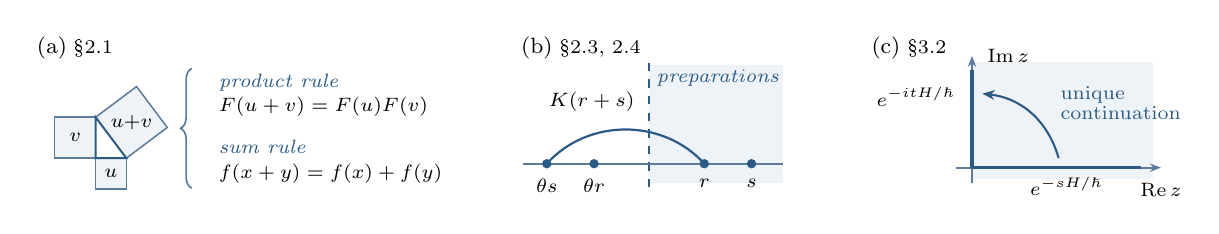
\begin{tikzpicture}[font=\footnotesize]
  % Panel (a): Pythagorean right triangle + 3 squares
  \begin{scope}[xshift=0cm]
    \node[anchor=west, font=\footnotesize] at (-0.35, 1.92) {(a) \scriptsize\S2.1};
    \coordinate (A) at (0.52, 0.52);
    \coordinate (B) at (0.91, 0.52);
    \coordinate (C) at (0.52, 1.04);
    \draw[fill=bandfill, draw=boxedge, line width=0.55pt] (A) -- (C) -- ($(C)+(-0.52,0)$) -- ($(A)+(-0.52,0)$) -- cycle;
    \node[font=\scriptsize] at (0.26, 0.78) {$v$};
    \draw[fill=bandfill, draw=boxedge, line width=0.55pt] (A) -- (B) -- ($(B)+(0,-0.39)$) -- ($(A)+(0,-0.39)$) -- cycle;
    \node[font=\scriptsize] at (0.715, 0.325) {$u$};
    \coordinate (D) at ($(C)+(0.52, 0.39)$);
    \coordinate (E) at ($(B)+(0.52, 0.39)$);
    \draw[fill=bandfill, draw=boxedge, line width=0.55pt] (B) -- (C) -- (D) -- (E) -- cycle;
    \node[font=\scriptsize] at (0.975, 0.975) {$u{+}v$};
    \draw[fill=white, draw=accent, line width=0.7pt] (A) -- (B) -- (C) -- cycle;
    \draw[decorate, decoration={brace, amplitude=4pt}, draw=accent!80, line width=0.6pt]
      (1.74, 0.14) -- (1.74, 1.66);
    \node[anchor=west, align=left, font=\scriptsize] at (1.96, 1.32)
      {\textit{\color{accent}product rule}\\[1pt]$F(u+v) = F(u)F(v)$};
    \node[anchor=west, align=left, font=\scriptsize] at (1.96, 0.48)
      {\textit{\color{accent}sum rule}\\[1pt]$f(x+y) = f(x)+f(y)$};
  \end{scope}

  % Panel (b): Reflection plane
  \begin{scope}[xshift=5.90cm]
    \node[anchor=west, font=\footnotesize] at (-0.1, 1.92) {(b) \scriptsize\S2.3, 2.4};
    \fill[bandfill] (1.65, 0.20) rectangle (3.35, 1.70);
    \draw[dashed, draw=accent, line width=0.7pt] (1.65, 0.15) -- (1.65, 1.76);
    \draw[draw=boxedge, line width=0.65pt] (0.05, 0.45) -- (3.35, 0.45);
    \node[font=\scriptsize\itshape, text=accent] at (2.52, 1.54) {preparations};
    \fill[accent] (0.35, 0.45) circle (1.7pt) node[below=2pt, font=\scriptsize, text=black] {$\theta s$};
    \fill[accent] (0.95, 0.45) circle (1.7pt) node[below=2pt, font=\scriptsize, text=black] {$\theta r$};
    \fill[accent] (2.35, 0.45) circle (1.7pt) node[below=2pt, font=\scriptsize, text=black] {$r$};
    \fill[accent] (2.95, 0.45) circle (1.7pt) node[below=2pt, font=\scriptsize, text=black] {$s$};
    \draw[draw=accent, line width=0.8pt] (0.35, 0.45) to[bend left=48] (2.35, 0.45);
    \node[font=\scriptsize, text=black, inner sep=1pt] at (0.92, 1.24) {$K(r+s)$};
  \end{scope}

  % Panel (c): Right half-plane continuation
  \begin{scope}[xshift=10.50cm]
    \node[anchor=west, font=\footnotesize] at (-0.25, 1.92) {(c) \scriptsize\S3.2};
    \fill[bandfill] (1.15, 0.25) rectangle (3.45, 1.74);
    \draw[-{Stealth[length=4pt,width=3pt]}, draw=boxedge, line width=0.65pt] (1.15, 0.20) -- (1.15, 1.82) node[right=2pt, font=\scriptsize, text=black] {$\ImPart z$};
    \draw[-{Stealth[length=4pt,width=3pt]}, draw=boxedge, line width=0.65pt] (0.95, 0.40) -- (3.55, 0.40) node[below=2pt, font=\scriptsize, text=black] {$\RePart z$};
    \draw[draw=accent, line width=1.1pt] (1.15, 0.40) -- (3.30, 0.40);
    \draw[draw=accent, line width=1.1pt] (1.15, 0.40) -- (1.15, 1.64);
    \node[font=\scriptsize] at (2.35, 0.16) {$e^{-sH/\hbar}$};
    \node[anchor=east, font=\scriptsize] at (1.06, 1.30) {$e^{-itH/\hbar}$};
    \draw[-{Stealth[length=4.5pt,width=3.5pt]}, draw=accent, line width=0.75pt]
      (2.25, 0.52) to[bend right=34] (1.28, 1.34);
    \node[anchor=west, align=left, font=\scriptsize, text=accent] at (2.15, 1.22) {unique\\[-1pt]continuation};
  \end{scope}
\end{tikzpicture}
\vspace{-0.5em}
\caption{\small (a) Pythagoras~(1), read twice. (b) Reflection $\theta$ pairs pulses at $r$ and $s$ by $K(r+s)$. (c) The shift $e^{-sH/\hbar}$ continues uniquely into $\RePart z > 0$, with unitary boundary $e^{-itH/\hbar}$.}
\vspace{-0.4em}
\end{figure}

\section{The law and the operator}

\noindent\textbf{2.1\enspace Pythagoras.} Squared lengths of orthogonal displacements add. The rules give readings the same geometry. The sum rule makes expectation linear, normalized and nonnegative on squares, so $\langle X, Y\rangle = \E[XY]$ is a positive inner product on centred readings. The product rule makes independent centred readings orthogonal, $\E[XY] = \E[X]\E[Y] = 0$, so their squared lengths add:
\begin{equation}
  \|X + Y\|^2 = \|X\|^2 + \|Y\|^2.
\end{equation}
The rules and the axiom meet in this one equation, and it is read twice (Figure~2a): with the product rule it gives the law (\S2.2), with the sum rule the Born rule (\S3.5).

\medskip
\noindent\textbf{2.2\enspace The law.} Let $C = \hbar A^{-1}$ be the covariance of the law, $A/\hbar$ its precision. For a finite list of tests $f_i$, linearity $\sum_i \xi_i\Phi(f_i) = \Phi(\sum_i \xi_i f_i)$ reduces the joint characteristic function to one reading $\E e^{i\Phi(f)}$ at $f = \sum_i \xi_i f_i$. Put $G_{ij} = \langle f_i, A^{-1} f_j\rangle$, removing null directions, so $\Phi(f)$ has squared length $\hbar u$ with $u = \xi^{\mathsf{T}} G \xi$. Equal values for the isometries of this form make $\E e^{i\Phi(f)} = F(u)$ radial; marginal consistency, the sum rule, gives the same $F$ for every list. Readings of two independent copies, with forms $u$ and $v$, are orthogonal (\S2.1), so their sum has squared length $\hbar(u+v)$; the rotations that mix the copies are isometries too, and the product rule multiplies their characteristic functions. Thus
\begin{equation}
  F(u + v) = F(u)F(v), \qquad F(0) = 1, \qquad F(u) = e^{-\hbar u/2}.
\end{equation}
Indeed $F$ is real ($\xi \mapsto -\xi$) and $F(u) = F(u/2)^2 \ge 0$; continuity excludes zeros, so $\log F$ is real, additive and nonpositive ($|F| \le 1$). The variance $\hbar u$ fixes $F'(0) = -\hbar/2$. Fourier inversion then determines every finite joint law given $A$. Two independent fair signs show the force of this: the first coordinate never vanishes, yet a $45^\circ$ rotation zeros it half the time, failing the isometry test.

\vspace{3pt}
\noindent\textbf{2.3\enspace Locality and reflection positivity.} The law~(2) leaves $A$ open. On a finite lattice of $N$ sites with graph Laplacian $L = B^{\mathsf{T}}B$ (eigenvalues $\ell_1,\dots,\ell_N$, not all equal), fix the site and edge-difference mean squares $\tr C = S > 0$ and $\tr(LC) = rS$, with interior ratio $\ell_{\min} < r < \ell_{\max}$. Gaussian differential entropy is $\frac{1}{2}\log\det C + \text{const}$ (maximal at fixed covariance). Stationarity gives $C^{-1} = \alpha I + \beta L$: Rolle's theorem on $\prod_i(1 + t(\ell_i - r))$ gives a unique positive-definite solution, and whitening any rival $C'$ with $\log x \le x - 1$ proves strict global optimality among positive-definite matrices with the same two traces. With $w_i = (\alpha + \beta\ell_i)^{-1}$ and $\bar\ell = \tr(L)/N$, the constraints $\sum_i w_i = S$, $\sum_i \ell_i w_i = rS$ and $(\alpha + \beta r)S = N$ yield the stiffness identity
\begin{equation*}
  N(\bar\ell - r) = \beta \sum_{i=1}^N w_i(\ell_i - r)^2.
\end{equation*}
So $\beta > 0$ exactly when $r < \bar\ell$, readings smoother than white noise, and the constant mode $\ell_1 = 0$ forces $\alpha > 0$: then $\hbar = 1/\beta > 0$ and $m^2 = \alpha/\beta > 0$. In continuum notation the unnormalized lattice density is
\begin{equation}
  \exp\!\left(-\frac{1}{2\hbar}\int\bigl(|\nabla\varphi|_g^2 + m^2\varphi^2\bigr)\right).
\end{equation}
At mesh $a$, use site coordinates $a^{D/2}\varphi_i$ and $B = a^{-1}B_0$, where $B_0$ is the ordinary site-to-edge incidence matrix. Let $a \downarrow 0$ on exhausting free boxes, holding the inferred $m, \hbar > 0$ fixed: finite-difference consistency on smeared tests and the uniform inverse bound $m^{-2}$ give convergence of the free-box covariances, hence convergence of the finite joint Gaussian laws, to the centred Gaussian law~(2) with $A = -\Delta_g + m^2$ (covariance $\hbar(-\Delta_g + m^2)^{-1}$, precision local and of degree one in $-\Delta_g$).

In a free lattice box symmetric about the plane through sites at $s = 0$ (normal coordinate $s$, reflection $\theta: s \mapsto -s$), fixing the plane field splits the exponent of~(3) into a term for each half, so by the product rule the two halves are independent given that field, and reflection exchanges them. A real \textit{preparation} $X$, a function of readings at $s > 0$, paired with its reflection therefore has squared length
\begin{equation}
  \langle\theta X, X\rangle = \E[\theta X \cdot X] = \E\bigl[(\E[X \mid \text{plane}])^2\bigr] \ge 0.
\end{equation}
This inequality survives the continuum limit (verified directly in~\S2.4). For \textit{pulses}, tests concentrated at $s_i > 0$ with strengths $c_i$, it reads $\sum_{i,j} c_i c_j K(s_i + s_j) \ge 0$, where $K(\tau)$ is the covariance of two pulses at normal separation $\tau$ (Figure~2b).

\vspace{3pt}
\noindent\textbf{2.4\enspace The operator.} Conversely, no local invariant precision of higher degree passes the reflected test~(4).
\newpage
\noindent Translation invariance makes the coefficients of a local finite-order differential precision constant; rotating any $p$ to the first axis leaves an even polynomial in $p_1$, so orthogonal invariance makes the Fourier symbol a polynomial $P(|p|_g^2)$. Like the precision of~\S2.3 it is positive with a gap: $P(x) > 0$ for $x \ge 0$. Fix a transverse momentum $k \in \R^{D-1}$, leaving normal momentum $q \in \R$, and let $K_k(r)$ be the inverse Fourier transform of $1/P(q^2 + |k|^2)$. Reflection pairs pulses at $r, s > 0$ by $K_k(r + s)$. For the squared operator, $P(x) = (x + m^2)^2$, the normalized kernel is $\kappa(r) = (1 + \omega_k|r|)e^{-\omega_k|r|}$, with $\omega_k = \sqrt{|k|^2 + m^2}$. For distinct pulse positions its Gram determinant is
\begin{equation}
  \kappa(2r)\kappa(2s) - \kappa(r + s)^2 = -\omega_k^2(r - s)^2 e^{-2\omega_k(r+s)}.
\end{equation}
One negative determinant rules out the square. One pair of opposite pulses, strengths $1, -1$ at $r, 2r$, rules out \textit{every} higher degree. With $u = qr$, the identity $\cos 2u - 2\cos 3u + \cos 4u = 2\cos 3u(\cos u - 1) = -u^2\cos 3u\,\sinc^2(u/2)$ ($\sinc x = \sin x / x$) is bounded by $u^2$; for $\deg P \ge 2$, dominated convergence gives
\begin{equation}
  \lim_{r\to 0^+}\frac{K_k(2r) - 2K_k(3r) + K_k(4r)}{r^2}
  = -\int_{\R}\frac{q^2}{P(q^2 + |k|^2)}\,\frac{\dd q}{2\pi} < 0.
\end{equation}
Smearing narrowly in $s > 0$ and transversely with compact Fourier support keeps the reflected form strictly negative for an actual test function. Degree zero gives no coupling between separated points. Degree one is not an assumption: it is the only nonconstant degree that survives the reflected test. Positivity on $x \ge 0$ leaves $P(x) = b(x + m^2)$, $b, m > 0$, with $b$ absorbed in $\hbar$: this is~(3). Its kernel $K_k(r+s) = e^{-\omega_k(r+s)}/(2\omega_k) = K_k(r)K_k(s)/K_k(0)$ factors through the plane: given the plane the two sides are uncorrelated, hence independent, giving~(4) in the continuum.

\section{The quantum structure}

\noindent\textbf{3.1\enspace States.} The reflected overlaps $\langle \theta\bar{X}, X'\rangle$ fix the squared norm of every finite linear combination of preparations, so quotienting zero-norm combinations and completing determines the minimal complex state space $\HH$ uniquely up to a label-preserving unitary. By~(4), conditioning $[X] \mapsto \E[X \mid \text{plane}]$ embeds $\HH$ isometrically into plane $L^2$: a state is what the plane knows of its preparation. The kernel $K_k$ makes positive-time mollifications of each spatial smear Cauchy in mean square; their limits are the plane readings. The corresponding plane characters are limits of conditioned preparations and are total in plane $L^2$ by finite-dimensional Fourier uniqueness, so conditioning is onto. Use unitary Fourier conventions transversely. In the complexification of the real test space the reflected covariance is an ordinary inner product of the features $Jf$ in the one-particle space $\hh$,
\begin{equation}
  (Jf)(k) = \sqrt{\frac{\hbar}{2\omega_k}}\int_0^\infty e^{-s\omega_k}\hat{f}(s, k)\,\dd s,
  \qquad
  C(\theta\bar{f}, f') = \langle Jf, Jf'\rangle_{\hh},
  \qquad
  \hh = L^2(\dd k; \C).
\end{equation}
The range is dense: a fixed nonnegative bump in $s$ has a strictly positive Laplace transform, so it divides out on each compact momentum set.

The Gaussian law now fixes inner products of nonlinear readings as well. For a real test $f$ supported in $s > 0$, form the complex Wick exponential $W(f) = \exp(i\Phi(f) + C(f,f)/2)$. Evaluating~(2) at $f' - \theta f$ gives the reflected overlap $\langle\theta\overline{W(f)}, W(f')\rangle = \exp\langle Jf, Jf'\rangle$. Expanding the exponential gives the inner products of
\begin{equation}
  \varepsilon(u) = \bigoplus_{n\ge 0}\frac{u^{\otimes n}}{\sqrt{n!}}
  \quad\text{in}\quad
  \HH = \bigoplus_{n\ge 0}\hh^{\otimes_s n}.
\end{equation}
The tensors are symmetric and the $n!$ is the exponential's: the excitations are identical bosons. By Fourier inversion on each finite list of readings, the classes $[W(f)]$ span densely, and derivatives of $\varepsilon(tu)$ give the symmetric tensors by polarization. By Gram uniqueness, $[W(f)] \mapsto \varepsilon(iJf)$ is the unique label-preserving unitary identifying $\HH$ with Fock space. On any nonzero feature $u = iJf$, the states at $0, u, \dots, (n-1)u$ have Gram matrix $(\exp(j\ell\|u\|^2))$ ($0 \le j, \ell < n$), a Vandermonde matrix in $e^{j\|u\|^2}$ with nonzero determinant for every $n$, proving $\dim\HH = \infty$; continuity of $u \mapsto \varepsilon(u)$ transfers separability from $\hh$ to $\HH$.

\vspace{3pt}
\noindent\textbf{3.2\enspace Evolution.} A shift by $s$ multiplies $Jf$ by $e^{-s\omega_k}$, continuing uniquely into $\RePart z > 0$ as $e^{-z\omega_k}$ with unitary imaginary boundary (Figure~2c). On the $n$-particle sector phases multiply, giving
\begin{equation}
  U(t) = e^{-itH/\hbar}, \qquad H_n = \hbar\sum_{j=1}^n \omega_{k_j}, \qquad i\hbar\dot\psi = H\psi \quad \text{on } \Dom H.
\end{equation}
A particle of momentum $p = \hbar k$ has energy $E(p) = \hbar\omega_k$: Einstein's relation $E(p)^2 = |p|_g^2 + M^2$ is Pythagoras once more, rest mass $M = \hbar m$ (at rest, $E = Mc^2$ in ordinary units); sums stay in the forward cone. Removing the rest-energy phase and scaling $p = \varepsilon p_0$, $t = \tau/\varepsilon^2$ gives $(E(\varepsilon p_0) - M)/\varepsilon^2 \to |p_0|_g^2/(2M)$: on each fixed rescaled $L^2$ wave packet, one-particle evolution converges to the free nonrelativistic Schr\"odinger evolution.

For a real Schwartz plane test $h$ with $\|h\|_2 = 1$, the plane reading $Q(h)$ and its time derivative $P(h) = \dot{Q}(h)$ obey $[Q(h), P(h)] = i\hbar I$ on the finite-particle domain: plane readings commute, the shift does not. Particle-number cutoffs tapering from $N$ to $2N$ have adjacent differences $O(N^{-1})$, so the $O(\sqrt{N})$ creation and annihilation bounds make the cutoff commutators tend to zero; thus the weak commutator identity extends to $\Dom Q \cap \Dom P$, where the $2\times 2$ Gram determinant gives Heisenberg's uncertainty bound $\Delta Q\,\Delta P \ge \hbar/2$. Time is not assumed: $t$ is the imaginary part of the continued distance $z = s + it$. Because $H_n \ge n\hbar m$, the spectrum of $H$ lies in $\{0\} \cup [\hbar m, \infty)$, so the vacuum $\varepsilon(0)$, alone at zero, is unique, with a mass gap $\hbar m$. Energy over $\hbar$ is the rate at which the plane forgets a receding preparation, and $m$ is the slowest such rate.

\newpage
\setlength{\intextsep}{7pt plus 2pt minus 2pt}
\noindent\textbf{3.3\enspace Special relativity.} A rotation by $\vartheta$ in a plane containing the normal continues, at $z = s \to it$ and $\vartheta = i\eta$, to a boost of rapidity $\eta$. Boosts preserve $\dd k/2\omega_k$ in~(7), so they act unitarily and $t$ is the time of the Poincar\'e group. The continued field $\Phi(f) = c^*(u_f) + c(u_{\bar{f}})$ creates $u_f$ and removes $u_{\bar{f}}$, where $u_f$ is~(7) with $e^{it\omega_k}$ in place of $e^{-s\omega_k}$ and $t$ over $\R$; it is an operator-valued tempered distribution with cyclic vacuum. The heat kernel writes the Euclidean two-point function at separation $(z, x)$ as $G_E(z^2 + |x|_g^2)$, with $G_E(w) \propto \int_0^\infty \lambda^{-D/2} e^{-m^2\lambda - w/(4\lambda)}\,\dd\lambda$ holomorphic for $\RePart w > 0$. On compact spacelike sets ($|x|_g > |t|$), both boundary values $z = \varepsilon \pm it \to \pm it$ ($\varepsilon \downarrow 0^+$) converge uniformly to $G_E(|x|_g^2 - t^2)$, so the commutator $[\Phi(f), \Phi(f')] = (\langle u_{\bar{f}}, u_{f'}\rangle - \langle u_{\bar{f}'}, u_f\rangle)I$ vanishes there as a distribution. The continued form $|x|_g^2 - t^2$ has null cone $|x|_g = |t|$, so the invariant speed is finite and nonzero: $1$ in units of $g$.

\vspace{1.5pt}
\noindent\textbf{3.4\enspace Composition.} By the product rule the plane laws $\mu_1$, $\mu_2$ of independent systems $1$, $2$ multiply, giving $L^2(\mu_1 \otimes \mu_2) \simeq \HH_1 \otimes \HH_2$; in Fock form $\hh_{12} = \hh_1 \oplus \hh_2$ and $\varepsilon(u \oplus v) \mapsto \varepsilon(u) \otimes \varepsilon(v)$ is unitary.

\vspace{1.5pt}
\noindent\textbf{3.5\enspace Sharp probabilities.} A sharp \textit{event} is a projection $P$; the sum rule and equal values govern its weight $p_\psi(P)$ in a unit state $\psi$. By~\S3.1, $\HH$ is infinite dimensional and separable. By unitary invariance every rank-one event perpendicular to $\psi$ has the same weight; arbitrarily many are mutually orthogonal, so that weight is zero. Countable additivity extends this to their closed spans. For any $P$, the part of its range perpendicular to $P\psi$ is perpendicular to $\psi$, so its weight vanishes.

The remaining ray and $\psi$ are classified up to unitaries fixing $\psi$ by their squared overlap $x = \|P\psi\|^2 \in [0, 1]$, so $p_\psi(P) = f(x)$ with $f(1) = 1$. Three orthogonal directions realize every split $x + y \le 1$, so Pythagoras and additivity give $f(x + y) = f(x) + f(y)$. Putting $d(x) = f(x) - x$, complement symmetry gives $d(1 - x) = -d(x)$, and doubling gives $2d(x) = d(2x)$ for $x \le \frac{1}{2}$ and $2d(x) = -2d(1 - x) = -d(2 - 2x) = d(2x - 1)$ for $x > \frac{1}{2}$, so $2d(x) \in d([0, 1])$. Since $f \le 1$, $M = \sup_{[0,1]} d < \infty$ satisfies $M \le M/2$, giving $d \le 0$ and by symmetry $d = 0$:
\begin{equation}
  f(x + y) = f(x) + f(y), \qquad f(1) = 1, \qquad f(x) = x.
\end{equation}
Conversely these weights add by Pythagoras. Vector states are rays, normal mixtures are density operators, and projection-valued measures $P$ on $\R$ give self-adjoint observables $A = \int a\,\dd P(a)$ on $\Dom A$.

\vspace{1.5pt}
\noindent\textbf{3.6\enspace Ideal conditioning.} For a density operator $\rho$, write $p(P) = \tr(\rho P) > 0$. Certainty of $P$ supports the conditional state on its range. By the product rule its value on each subprojection $Q \le P$ must be $p(Q)/p(P)$. Rank-one subprojections fix all matrix elements by polarization, giving uniquely the L\"uders projection update
\begin{equation}
  \rho_P = \frac{P\rho P}{\tr(\rho P)}, \qquad \psi_P = \frac{P\psi}{\|P\psi\|},
\end{equation}
with the ray update on the right for a pure state $\psi$ ($P\psi \ne 0$).

\section{The axioms}

Under the stated rules, the reflected readings determine the quantum structure in Table~1. The Osterwalder--Schrader axioms, the Euclidean form of Wightman's, hold for the continuum law of~\S2.3; \S3.1--3.3 are their reconstruction, here one conditional expectation and one continuation. Table~1 records where each axiom is established.

\begin{table}[h]
\vspace{-0.15em}
\centering
\small
\renewcommand{\arraystretch}{0.88}
\begin{tabular}{@{}l@{\qquad}l@{\hspace{3.2em}}l@{\qquad}l@{}}
\toprule
\textbf{von Neumann} & & \textbf{Wightman} & \\
\midrule
Hilbert space & \S3.1 & Poincar\'e covariance & \S3.3 \\
Unitary evolution & \S3.2 & Forward-cone spectrum & \S3.2 \\
Tensor product & \S3.4 & Unique vacuum & \S3.2 \\
Born rule & \S3.5 & Field distributions & \S3.3 \\
Self-adjoint observables & \S3.5 & Spacelike commutativity & \S3.3 \\
Projection update & \S3.6 & Cyclic vacuum & \S3.3 \\
\bottomrule
\end{tabular}
\vspace{-0.15em}
\caption{\small The axioms and where each is established.}
\vspace{-0.25em}
\end{table}

The law determined here is free. More generally, reflection and shift invariance and conditional independence given the plane give (4) and the state space. Continuous shifts on smeared readings give the evolution; independent products give composition. The Born rule and the update use the state space and the stated probability rules, not the field law.

\section{One equation}

The same composition principle appears four times, in two forms:
\begin{equation}
  \phi(a + b) = \phi(a)\,\phi(b) \quad (\text{product rule}),
  \qquad
  \phi(a + b) = \phi(a) + \phi(b) \quad (\text{sum rule}).
\end{equation}
For a product solution with $0 < \phi \le 1$ and $\phi(a) < 1$, the function $x \mapsto \log\phi(ax)/\log\phi(a)$ is an additive solution on $[0, 1]$ with values in $[0, 1]$ and value $1$ at $1$, so the doubling-map proof of~\S3.5 solves both. Squared lengths add and laws multiply: the Gaussian law~(2). Distances add and normalized kernels multiply: the kernel $K_k/K_k(0)$ of~\S2.4, with it the shift and the evolution~(9). Systems add and state spaces multiply: the tensor product of~\S3.4. Squared overlaps add and so do probabilities: the Born rule~(10).

Under these rules, only $m$ and $\hbar$ remain free.

\par\vspace{1.5pt}
{\small\noindent\textbf{Acknowledgments.} This work used the Logos AI system, incorporating several frontier models. The Lean formalisation used GPT 6.2 Astra and Gemini Neon.\par}
\end{document}
